
% Default to the notebook output style

    


% Inherit from the specified cell style.




    
\documentclass[11pt]{article}

    
    
    \usepackage[T1]{fontenc}
    % Nicer default font (+ math font) than Computer Modern for most use cases
    \usepackage{mathpazo}

    % Basic figure setup, for now with no caption control since it's done
    % automatically by Pandoc (which extracts ![](path) syntax from Markdown).
    \usepackage{graphicx}
    % We will generate all images so they have a width \maxwidth. This means
    % that they will get their normal width if they fit onto the page, but
    % are scaled down if they would overflow the margins.
    \makeatletter
    \def\maxwidth{\ifdim\Gin@nat@width>\linewidth\linewidth
    \else\Gin@nat@width\fi}
    \makeatother
    \let\Oldincludegraphics\includegraphics
    % Set max figure width to be 80% of text width, for now hardcoded.
    \renewcommand{\includegraphics}[1]{\Oldincludegraphics[width=.8\maxwidth]{#1}}
    % Ensure that by default, figures have no caption (until we provide a
    % proper Figure object with a Caption API and a way to capture that
    % in the conversion process - todo).
    \usepackage{caption}
    \DeclareCaptionLabelFormat{nolabel}{}
    \captionsetup{labelformat=nolabel}

    \usepackage{adjustbox} % Used to constrain images to a maximum size 
    \usepackage{xcolor} % Allow colors to be defined
    \usepackage{enumerate} % Needed for markdown enumerations to work
    \usepackage{geometry} % Used to adjust the document margins
    \usepackage{amsmath} % Equations
    \usepackage{amssymb} % Equations
    \usepackage{textcomp} % defines textquotesingle
    % Hack from http://tex.stackexchange.com/a/47451/13684:
    \AtBeginDocument{%
        \def\PYZsq{\textquotesingle}% Upright quotes in Pygmentized code
    }
    \usepackage{upquote} % Upright quotes for verbatim code
    \usepackage{eurosym} % defines \euro
    \usepackage[mathletters]{ucs} % Extended unicode (utf-8) support
    \usepackage[utf8x]{inputenc} % Allow utf-8 characters in the tex document
    \usepackage{fancyvrb} % verbatim replacement that allows latex
    \usepackage{grffile} % extends the file name processing of package graphics 
                         % to support a larger range 
    % The hyperref package gives us a pdf with properly built
    % internal navigation ('pdf bookmarks' for the table of contents,
    % internal cross-reference links, web links for URLs, etc.)
    \usepackage{hyperref}
    \usepackage{longtable} % longtable support required by pandoc >1.10
    \usepackage{booktabs}  % table support for pandoc > 1.12.2
    \usepackage[inline]{enumitem} % IRkernel/repr support (it uses the enumerate* environment)
    \usepackage[normalem]{ulem} % ulem is needed to support strikethroughs (\sout)
                                % normalem makes italics be italics, not underlines
    

    
    
    % Colors for the hyperref package
    \definecolor{urlcolor}{rgb}{0,.145,.698}
    \definecolor{linkcolor}{rgb}{.71,0.21,0.01}
    \definecolor{citecolor}{rgb}{.12,.54,.11}

    % ANSI colors
    \definecolor{ansi-black}{HTML}{3E424D}
    \definecolor{ansi-black-intense}{HTML}{282C36}
    \definecolor{ansi-red}{HTML}{E75C58}
    \definecolor{ansi-red-intense}{HTML}{B22B31}
    \definecolor{ansi-green}{HTML}{00A250}
    \definecolor{ansi-green-intense}{HTML}{007427}
    \definecolor{ansi-yellow}{HTML}{DDB62B}
    \definecolor{ansi-yellow-intense}{HTML}{B27D12}
    \definecolor{ansi-blue}{HTML}{208FFB}
    \definecolor{ansi-blue-intense}{HTML}{0065CA}
    \definecolor{ansi-magenta}{HTML}{D160C4}
    \definecolor{ansi-magenta-intense}{HTML}{A03196}
    \definecolor{ansi-cyan}{HTML}{60C6C8}
    \definecolor{ansi-cyan-intense}{HTML}{258F8F}
    \definecolor{ansi-white}{HTML}{C5C1B4}
    \definecolor{ansi-white-intense}{HTML}{A1A6B2}

    % commands and environments needed by pandoc snippets
    % extracted from the output of `pandoc -s`
    \providecommand{\tightlist}{%
      \setlength{\itemsep}{0pt}\setlength{\parskip}{0pt}}
    \DefineVerbatimEnvironment{Highlighting}{Verbatim}{commandchars=\\\{\}}
    % Add ',fontsize=\small' for more characters per line
    \newenvironment{Shaded}{}{}
    \newcommand{\KeywordTok}[1]{\textcolor[rgb]{0.00,0.44,0.13}{\textbf{{#1}}}}
    \newcommand{\DataTypeTok}[1]{\textcolor[rgb]{0.56,0.13,0.00}{{#1}}}
    \newcommand{\DecValTok}[1]{\textcolor[rgb]{0.25,0.63,0.44}{{#1}}}
    \newcommand{\BaseNTok}[1]{\textcolor[rgb]{0.25,0.63,0.44}{{#1}}}
    \newcommand{\FloatTok}[1]{\textcolor[rgb]{0.25,0.63,0.44}{{#1}}}
    \newcommand{\CharTok}[1]{\textcolor[rgb]{0.25,0.44,0.63}{{#1}}}
    \newcommand{\StringTok}[1]{\textcolor[rgb]{0.25,0.44,0.63}{{#1}}}
    \newcommand{\CommentTok}[1]{\textcolor[rgb]{0.38,0.63,0.69}{\textit{{#1}}}}
    \newcommand{\OtherTok}[1]{\textcolor[rgb]{0.00,0.44,0.13}{{#1}}}
    \newcommand{\AlertTok}[1]{\textcolor[rgb]{1.00,0.00,0.00}{\textbf{{#1}}}}
    \newcommand{\FunctionTok}[1]{\textcolor[rgb]{0.02,0.16,0.49}{{#1}}}
    \newcommand{\RegionMarkerTok}[1]{{#1}}
    \newcommand{\ErrorTok}[1]{\textcolor[rgb]{1.00,0.00,0.00}{\textbf{{#1}}}}
    \newcommand{\NormalTok}[1]{{#1}}
    
    % Additional commands for more recent versions of Pandoc
    \newcommand{\ConstantTok}[1]{\textcolor[rgb]{0.53,0.00,0.00}{{#1}}}
    \newcommand{\SpecialCharTok}[1]{\textcolor[rgb]{0.25,0.44,0.63}{{#1}}}
    \newcommand{\VerbatimStringTok}[1]{\textcolor[rgb]{0.25,0.44,0.63}{{#1}}}
    \newcommand{\SpecialStringTok}[1]{\textcolor[rgb]{0.73,0.40,0.53}{{#1}}}
    \newcommand{\ImportTok}[1]{{#1}}
    \newcommand{\DocumentationTok}[1]{\textcolor[rgb]{0.73,0.13,0.13}{\textit{{#1}}}}
    \newcommand{\AnnotationTok}[1]{\textcolor[rgb]{0.38,0.63,0.69}{\textbf{\textit{{#1}}}}}
    \newcommand{\CommentVarTok}[1]{\textcolor[rgb]{0.38,0.63,0.69}{\textbf{\textit{{#1}}}}}
    \newcommand{\VariableTok}[1]{\textcolor[rgb]{0.10,0.09,0.49}{{#1}}}
    \newcommand{\ControlFlowTok}[1]{\textcolor[rgb]{0.00,0.44,0.13}{\textbf{{#1}}}}
    \newcommand{\OperatorTok}[1]{\textcolor[rgb]{0.40,0.40,0.40}{{#1}}}
    \newcommand{\BuiltInTok}[1]{{#1}}
    \newcommand{\ExtensionTok}[1]{{#1}}
    \newcommand{\PreprocessorTok}[1]{\textcolor[rgb]{0.74,0.48,0.00}{{#1}}}
    \newcommand{\AttributeTok}[1]{\textcolor[rgb]{0.49,0.56,0.16}{{#1}}}
    \newcommand{\InformationTok}[1]{\textcolor[rgb]{0.38,0.63,0.69}{\textbf{\textit{{#1}}}}}
    \newcommand{\WarningTok}[1]{\textcolor[rgb]{0.38,0.63,0.69}{\textbf{\textit{{#1}}}}}
    
    
    % Define a nice break command that doesn't care if a line doesn't already
    % exist.
    \def\br{\hspace*{\fill} \\* }
    % Math Jax compatability definitions
    \def\gt{>}
    \def\lt{<}
    % Document parameters
    \title{Uni\_Template\_V1.1}
    
    
    

    % Pygments definitions
    
\makeatletter
\def\PY@reset{\let\PY@it=\relax \let\PY@bf=\relax%
    \let\PY@ul=\relax \let\PY@tc=\relax%
    \let\PY@bc=\relax \let\PY@ff=\relax}
\def\PY@tok#1{\csname PY@tok@#1\endcsname}
\def\PY@toks#1+{\ifx\relax#1\empty\else%
    \PY@tok{#1}\expandafter\PY@toks\fi}
\def\PY@do#1{\PY@bc{\PY@tc{\PY@ul{%
    \PY@it{\PY@bf{\PY@ff{#1}}}}}}}
\def\PY#1#2{\PY@reset\PY@toks#1+\relax+\PY@do{#2}}

\expandafter\def\csname PY@tok@gd\endcsname{\def\PY@tc##1{\textcolor[rgb]{0.63,0.00,0.00}{##1}}}
\expandafter\def\csname PY@tok@gu\endcsname{\let\PY@bf=\textbf\def\PY@tc##1{\textcolor[rgb]{0.50,0.00,0.50}{##1}}}
\expandafter\def\csname PY@tok@gt\endcsname{\def\PY@tc##1{\textcolor[rgb]{0.00,0.27,0.87}{##1}}}
\expandafter\def\csname PY@tok@gs\endcsname{\let\PY@bf=\textbf}
\expandafter\def\csname PY@tok@gr\endcsname{\def\PY@tc##1{\textcolor[rgb]{1.00,0.00,0.00}{##1}}}
\expandafter\def\csname PY@tok@cm\endcsname{\let\PY@it=\textit\def\PY@tc##1{\textcolor[rgb]{0.25,0.50,0.50}{##1}}}
\expandafter\def\csname PY@tok@vg\endcsname{\def\PY@tc##1{\textcolor[rgb]{0.10,0.09,0.49}{##1}}}
\expandafter\def\csname PY@tok@vi\endcsname{\def\PY@tc##1{\textcolor[rgb]{0.10,0.09,0.49}{##1}}}
\expandafter\def\csname PY@tok@vm\endcsname{\def\PY@tc##1{\textcolor[rgb]{0.10,0.09,0.49}{##1}}}
\expandafter\def\csname PY@tok@mh\endcsname{\def\PY@tc##1{\textcolor[rgb]{0.40,0.40,0.40}{##1}}}
\expandafter\def\csname PY@tok@cs\endcsname{\let\PY@it=\textit\def\PY@tc##1{\textcolor[rgb]{0.25,0.50,0.50}{##1}}}
\expandafter\def\csname PY@tok@ge\endcsname{\let\PY@it=\textit}
\expandafter\def\csname PY@tok@vc\endcsname{\def\PY@tc##1{\textcolor[rgb]{0.10,0.09,0.49}{##1}}}
\expandafter\def\csname PY@tok@il\endcsname{\def\PY@tc##1{\textcolor[rgb]{0.40,0.40,0.40}{##1}}}
\expandafter\def\csname PY@tok@go\endcsname{\def\PY@tc##1{\textcolor[rgb]{0.53,0.53,0.53}{##1}}}
\expandafter\def\csname PY@tok@cp\endcsname{\def\PY@tc##1{\textcolor[rgb]{0.74,0.48,0.00}{##1}}}
\expandafter\def\csname PY@tok@gi\endcsname{\def\PY@tc##1{\textcolor[rgb]{0.00,0.63,0.00}{##1}}}
\expandafter\def\csname PY@tok@gh\endcsname{\let\PY@bf=\textbf\def\PY@tc##1{\textcolor[rgb]{0.00,0.00,0.50}{##1}}}
\expandafter\def\csname PY@tok@ni\endcsname{\let\PY@bf=\textbf\def\PY@tc##1{\textcolor[rgb]{0.60,0.60,0.60}{##1}}}
\expandafter\def\csname PY@tok@nl\endcsname{\def\PY@tc##1{\textcolor[rgb]{0.63,0.63,0.00}{##1}}}
\expandafter\def\csname PY@tok@nn\endcsname{\let\PY@bf=\textbf\def\PY@tc##1{\textcolor[rgb]{0.00,0.00,1.00}{##1}}}
\expandafter\def\csname PY@tok@no\endcsname{\def\PY@tc##1{\textcolor[rgb]{0.53,0.00,0.00}{##1}}}
\expandafter\def\csname PY@tok@na\endcsname{\def\PY@tc##1{\textcolor[rgb]{0.49,0.56,0.16}{##1}}}
\expandafter\def\csname PY@tok@nb\endcsname{\def\PY@tc##1{\textcolor[rgb]{0.00,0.50,0.00}{##1}}}
\expandafter\def\csname PY@tok@nc\endcsname{\let\PY@bf=\textbf\def\PY@tc##1{\textcolor[rgb]{0.00,0.00,1.00}{##1}}}
\expandafter\def\csname PY@tok@nd\endcsname{\def\PY@tc##1{\textcolor[rgb]{0.67,0.13,1.00}{##1}}}
\expandafter\def\csname PY@tok@ne\endcsname{\let\PY@bf=\textbf\def\PY@tc##1{\textcolor[rgb]{0.82,0.25,0.23}{##1}}}
\expandafter\def\csname PY@tok@nf\endcsname{\def\PY@tc##1{\textcolor[rgb]{0.00,0.00,1.00}{##1}}}
\expandafter\def\csname PY@tok@si\endcsname{\let\PY@bf=\textbf\def\PY@tc##1{\textcolor[rgb]{0.73,0.40,0.53}{##1}}}
\expandafter\def\csname PY@tok@s2\endcsname{\def\PY@tc##1{\textcolor[rgb]{0.73,0.13,0.13}{##1}}}
\expandafter\def\csname PY@tok@nt\endcsname{\let\PY@bf=\textbf\def\PY@tc##1{\textcolor[rgb]{0.00,0.50,0.00}{##1}}}
\expandafter\def\csname PY@tok@nv\endcsname{\def\PY@tc##1{\textcolor[rgb]{0.10,0.09,0.49}{##1}}}
\expandafter\def\csname PY@tok@s1\endcsname{\def\PY@tc##1{\textcolor[rgb]{0.73,0.13,0.13}{##1}}}
\expandafter\def\csname PY@tok@dl\endcsname{\def\PY@tc##1{\textcolor[rgb]{0.73,0.13,0.13}{##1}}}
\expandafter\def\csname PY@tok@ch\endcsname{\let\PY@it=\textit\def\PY@tc##1{\textcolor[rgb]{0.25,0.50,0.50}{##1}}}
\expandafter\def\csname PY@tok@m\endcsname{\def\PY@tc##1{\textcolor[rgb]{0.40,0.40,0.40}{##1}}}
\expandafter\def\csname PY@tok@gp\endcsname{\let\PY@bf=\textbf\def\PY@tc##1{\textcolor[rgb]{0.00,0.00,0.50}{##1}}}
\expandafter\def\csname PY@tok@sh\endcsname{\def\PY@tc##1{\textcolor[rgb]{0.73,0.13,0.13}{##1}}}
\expandafter\def\csname PY@tok@ow\endcsname{\let\PY@bf=\textbf\def\PY@tc##1{\textcolor[rgb]{0.67,0.13,1.00}{##1}}}
\expandafter\def\csname PY@tok@sx\endcsname{\def\PY@tc##1{\textcolor[rgb]{0.00,0.50,0.00}{##1}}}
\expandafter\def\csname PY@tok@bp\endcsname{\def\PY@tc##1{\textcolor[rgb]{0.00,0.50,0.00}{##1}}}
\expandafter\def\csname PY@tok@c1\endcsname{\let\PY@it=\textit\def\PY@tc##1{\textcolor[rgb]{0.25,0.50,0.50}{##1}}}
\expandafter\def\csname PY@tok@fm\endcsname{\def\PY@tc##1{\textcolor[rgb]{0.00,0.00,1.00}{##1}}}
\expandafter\def\csname PY@tok@o\endcsname{\def\PY@tc##1{\textcolor[rgb]{0.40,0.40,0.40}{##1}}}
\expandafter\def\csname PY@tok@kc\endcsname{\let\PY@bf=\textbf\def\PY@tc##1{\textcolor[rgb]{0.00,0.50,0.00}{##1}}}
\expandafter\def\csname PY@tok@c\endcsname{\let\PY@it=\textit\def\PY@tc##1{\textcolor[rgb]{0.25,0.50,0.50}{##1}}}
\expandafter\def\csname PY@tok@mf\endcsname{\def\PY@tc##1{\textcolor[rgb]{0.40,0.40,0.40}{##1}}}
\expandafter\def\csname PY@tok@err\endcsname{\def\PY@bc##1{\setlength{\fboxsep}{0pt}\fcolorbox[rgb]{1.00,0.00,0.00}{1,1,1}{\strut ##1}}}
\expandafter\def\csname PY@tok@mb\endcsname{\def\PY@tc##1{\textcolor[rgb]{0.40,0.40,0.40}{##1}}}
\expandafter\def\csname PY@tok@ss\endcsname{\def\PY@tc##1{\textcolor[rgb]{0.10,0.09,0.49}{##1}}}
\expandafter\def\csname PY@tok@sr\endcsname{\def\PY@tc##1{\textcolor[rgb]{0.73,0.40,0.53}{##1}}}
\expandafter\def\csname PY@tok@mo\endcsname{\def\PY@tc##1{\textcolor[rgb]{0.40,0.40,0.40}{##1}}}
\expandafter\def\csname PY@tok@kd\endcsname{\let\PY@bf=\textbf\def\PY@tc##1{\textcolor[rgb]{0.00,0.50,0.00}{##1}}}
\expandafter\def\csname PY@tok@mi\endcsname{\def\PY@tc##1{\textcolor[rgb]{0.40,0.40,0.40}{##1}}}
\expandafter\def\csname PY@tok@kn\endcsname{\let\PY@bf=\textbf\def\PY@tc##1{\textcolor[rgb]{0.00,0.50,0.00}{##1}}}
\expandafter\def\csname PY@tok@cpf\endcsname{\let\PY@it=\textit\def\PY@tc##1{\textcolor[rgb]{0.25,0.50,0.50}{##1}}}
\expandafter\def\csname PY@tok@kr\endcsname{\let\PY@bf=\textbf\def\PY@tc##1{\textcolor[rgb]{0.00,0.50,0.00}{##1}}}
\expandafter\def\csname PY@tok@s\endcsname{\def\PY@tc##1{\textcolor[rgb]{0.73,0.13,0.13}{##1}}}
\expandafter\def\csname PY@tok@kp\endcsname{\def\PY@tc##1{\textcolor[rgb]{0.00,0.50,0.00}{##1}}}
\expandafter\def\csname PY@tok@w\endcsname{\def\PY@tc##1{\textcolor[rgb]{0.73,0.73,0.73}{##1}}}
\expandafter\def\csname PY@tok@kt\endcsname{\def\PY@tc##1{\textcolor[rgb]{0.69,0.00,0.25}{##1}}}
\expandafter\def\csname PY@tok@sc\endcsname{\def\PY@tc##1{\textcolor[rgb]{0.73,0.13,0.13}{##1}}}
\expandafter\def\csname PY@tok@sb\endcsname{\def\PY@tc##1{\textcolor[rgb]{0.73,0.13,0.13}{##1}}}
\expandafter\def\csname PY@tok@sa\endcsname{\def\PY@tc##1{\textcolor[rgb]{0.73,0.13,0.13}{##1}}}
\expandafter\def\csname PY@tok@k\endcsname{\let\PY@bf=\textbf\def\PY@tc##1{\textcolor[rgb]{0.00,0.50,0.00}{##1}}}
\expandafter\def\csname PY@tok@se\endcsname{\let\PY@bf=\textbf\def\PY@tc##1{\textcolor[rgb]{0.73,0.40,0.13}{##1}}}
\expandafter\def\csname PY@tok@sd\endcsname{\let\PY@it=\textit\def\PY@tc##1{\textcolor[rgb]{0.73,0.13,0.13}{##1}}}

\def\PYZbs{\char`\\}
\def\PYZus{\char`\_}
\def\PYZob{\char`\{}
\def\PYZcb{\char`\}}
\def\PYZca{\char`\^}
\def\PYZam{\char`\&}
\def\PYZlt{\char`\<}
\def\PYZgt{\char`\>}
\def\PYZsh{\char`\#}
\def\PYZpc{\char`\%}
\def\PYZdl{\char`\$}
\def\PYZhy{\char`\-}
\def\PYZsq{\char`\'}
\def\PYZdq{\char`\"}
\def\PYZti{\char`\~}
% for compatibility with earlier versions
\def\PYZat{@}
\def\PYZlb{[}
\def\PYZrb{]}
\makeatother


    % Exact colors from NB
    \definecolor{incolor}{rgb}{0.0, 0.0, 0.5}
    \definecolor{outcolor}{rgb}{0.545, 0.0, 0.0}



    
    % Prevent overflowing lines due to hard-to-break entities
    \sloppy 
    % Setup hyperref package
    \hypersetup{
      breaklinks=true,  % so long urls are correctly broken across lines
      colorlinks=true,
      urlcolor=urlcolor,
      linkcolor=linkcolor,
      citecolor=citecolor,
      }
    % Slightly bigger margins than the latex defaults
    
    \geometry{verbose,tmargin=1in,bmargin=1in,lmargin=1in,rmargin=1in}
    
    

    \begin{document}
    
    
    \maketitle
    
    

    
    \begin{figure}
\centering

\includegraphics{img/logo1.png}
\caption{udlogo.png}
\end{figure}

    \begin{figure}
\centering
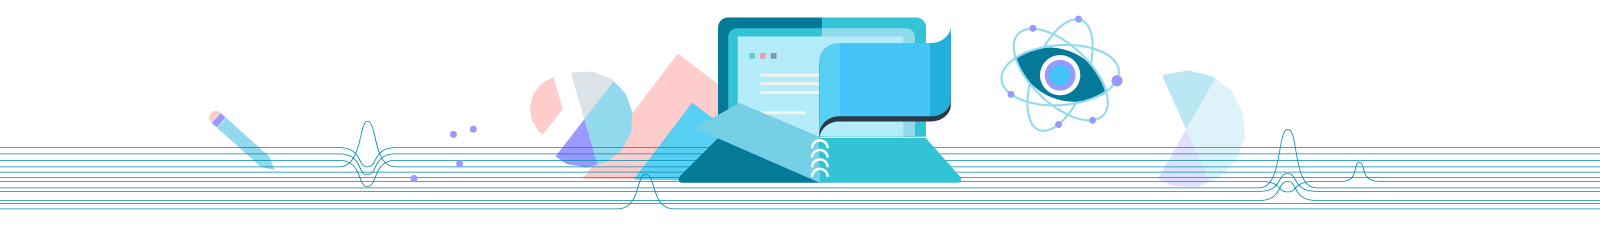
\includegraphics{img/logo3.png}
\caption{logo3.png}
\end{figure}

    版本号:1.1

作者:Jack Chen

协助:Jerry、Rita、ShuWen

更新日期:2018.12.17

    \begin{Verbatim}[commandchars=\\\{\}]
{\color{incolor}In [{\color{incolor}2}]:} \PY{k+kn}{import} \PY{n+nn}{os}
        \PY{k}{print}\PY{p}{(}\PY{n}{os}\PY{o}{.}\PY{n}{environ}\PY{p}{[}\PY{l+s+s1}{\PYZsq{}}\PY{l+s+s1}{PATH}\PY{l+s+s1}{\PYZsq{}}\PY{p}{]}\PY{p}{)}
\end{Verbatim}


    \begin{Verbatim}[commandchars=\\\{\}]
/Users/ctybz/Documents/anaconda2/bin:/anaconda3/bin:/Library/Frameworks/Python.framework/Versions/3.7/bin:/Library/Frameworks/Python.framework/Versions/2.7/bin:/Library/Frameworks/Python.framework/Versions/2.7/bin:/anaconda2/bin:/Library/Frameworks/Python.framework/Versions/2.7/bin:/usr/local/bin:/usr/bin:/bin:/usr/sbin:/sbin

    \end{Verbatim}

    \section{课程开发要点}\label{ux8bfeux7a0bux5f00ux53d1ux8981ux70b9}

\begin{enumerate}
\def\labelenumi{\arabic{enumi}.}
\item
  \textbf{课程结构}

  1.1 可以参照下方的课程架构部分

  1.2 关于时间设计,可以在习题的题干后面标注预估完成时间

  1.3 可以根据各课程的需要拓展教学板块
\item
  \textbf{形式}

  2.1 加粗:使用在课程重点内容的部分,用于强调其重要性
  用法:\textbf{TEXT}

  2.2
  字体、字号与颜色:用于不同模块的区分,例如:知识点环节的标题可以使用蓝色,举例子的环节可以使用紫色
  用法:color=\#0099ff size=72 face="黑体"

  2.3
  加载图片:多媒体的使用是增强课程趣味性的方法之一,因此在不侵犯他人版权的情况下可以适当配图进行说明,请注意本节课使用到的所有图片应该放置在同一个文件夹内,例如img,路径设置如下:
  
\includegraphics{img/logo1.png}

  2.4
  加载视频:同样的道理,导入视频也可以帮助学生理解内容,但需要注意视频是否能够正常播放,最好将视频放置在同一个文件夹中

  2.5 在【标记】状态下按右键可以选择一些表情作警告提示⚠️等作用

  2.6
  更多功能请访问官网文档:https://jupyter-notebook.readthedocs.io/en/latest/notebook.html
\item
  \textbf{LOGO}

  3.1
  在直播课中不使用Udacity教室,因此需要在大纲的开头和结尾都放上Udacity的LOGO
\item
  \textbf{打包与使用}

  4.1
  在完成了课件之后,应在notebook同一目录下创建一个文件夹,把所用到的图片、视频放在这个文件夹中,添加为压缩包

  4.2 最后分享给助教老师的课件形式应该是一个完整的压缩包
\end{enumerate}

    \section{课程架构}\label{ux8bfeux7a0bux67b6ux6784}

我将一节课的结构分为以下的不同步骤,你可以使用下面的链接来直接定位不同的部分
* Section \ref{step1}: 课程主题

\begin{itemize}
\item
  Section \ref{step1}: 上次课程回顾

  \begin{itemize}
  \tightlist
  \item
    Section \ref{step11}: 上节课知识点
  \item
    Section \ref{step12}: 上节课练习代码
  \item
    Section \ref{step13}: 上节课练习代码运行的效果
  \end{itemize}
\item
  Section \ref{step1}: 衔接过度到本节课的知识点主题
\item
  Section \ref{step3}: 新的知识点

  \begin{itemize}
  \tightlist
  \item
    Section \ref{step31}: 知识点的概念讲解
  \item
    Section \ref{step32}: 知识点的作用
  \item
    Section \ref{step33}: 知识点的语法结构
  \item
    Section \ref{step34}: 语法结构的讲解
  \end{itemize}
\item
  Section \ref{step4}: 习题

  \begin{itemize}
  \tightlist
  \item
    Section \ref{step41}: 当堂习题Section \ref{ex1}
  \item
    Section \ref{step42}: 当堂习题Section \ref{ex1_s}的解题思路与答案
  \end{itemize}
\item
  Section \ref{step5}: 课程内容总结
\item
  Section \ref{step6}: 优达课程资料
\item
  Section \ref{step7}: 作业内容与提交时间
\item
  Section \ref{step8}: 导师联系与答疑
\end{itemize}

     \# 本节课的主题

    【例】

\section{循环}\label{ux5faaux73af}

     \# 1. 课程回顾

     \#\# 1.1 回顾上节课知识点

    【例】在之前的章节中我们已经对\textbf{\emph{turtle}}模块非常熟悉了,可以使用forward()、left()等语法画出各种各样的图形,例如下面的代码将会画出一个\textbf{橙色}的正方形

     \#\# 1.2 回顾上节课练习内容 最好以代码形式呈现,代码需要良好的标注

    \begin{Verbatim}[commandchars=\\\{\}]
{\color{incolor}In [{\color{incolor} }]:} \PY{c+c1}{\PYZsh{} 【例】}
        \PY{k+kn}{import} \PY{n+nn}{turtle}
        \PY{k+kn}{import} \PY{n+nn}{os}
        
        \PY{c+c1}{\PYZsh{} 固定的turtle初始化过程}
        \PY{n}{jack} \PY{o}{=} \PY{n}{turtle}\PY{o}{.}\PY{n}{Turtle}\PY{p}{(}\PY{p}{)}
        \PY{n}{jack}\PY{o}{.}\PY{n}{color}\PY{p}{(}\PY{l+s+s1}{\PYZsq{}}\PY{l+s+s1}{orange}\PY{l+s+s1}{\PYZsq{}}\PY{p}{)}
        \PY{n}{jack}\PY{o}{.}\PY{n}{shape}\PY{p}{(}\PY{l+s+s1}{\PYZsq{}}\PY{l+s+s1}{turtle}\PY{l+s+s1}{\PYZsq{}}\PY{p}{)}
        
        \PY{c+c1}{\PYZsh{} 画出一条长为100的边}
        \PY{n}{jack}\PY{o}{.}\PY{n}{forward}\PY{p}{(}\PY{l+m+mi}{100}\PY{p}{)}
        \PY{c+c1}{\PYZsh{} 向左旋转90度}
        \PY{n}{jack}\PY{o}{.}\PY{n}{left}\PY{p}{(}\PY{l+m+mi}{90}\PY{p}{)}
        \PY{c+c1}{\PYZsh{} 重复3次画出一个4边形}
        \PY{n}{jack}\PY{o}{.}\PY{n}{forward}\PY{p}{(}\PY{l+m+mi}{100}\PY{p}{)}
        \PY{n}{jack}\PY{o}{.}\PY{n}{left}\PY{p}{(}\PY{l+m+mi}{90}\PY{p}{)}
        \PY{n}{jack}\PY{o}{.}\PY{n}{forward}\PY{p}{(}\PY{l+m+mi}{100}\PY{p}{)}
        \PY{n}{jack}\PY{o}{.}\PY{n}{left}\PY{p}{(}\PY{l+m+mi}{90}\PY{p}{)}
        \PY{n}{jack}\PY{o}{.}\PY{n}{forward}\PY{p}{(}\PY{l+m+mi}{100}\PY{p}{)}
        \PY{n}{jack}\PY{o}{.}\PY{n}{left}\PY{p}{(}\PY{l+m+mi}{90}\PY{p}{)}
        
        \PY{c+c1}{\PYZsh{} 正确地关闭程序}
        \PY{n}{turtle}\PY{o}{.}\PY{n}{done}\PY{p}{(}\PY{p}{)}
        \PY{n}{os}\PY{o}{.}\PY{n}{\PYZus{}exit}\PY{p}{(}\PY{l+m+mi}{0}\PY{p}{)}
\end{Verbatim}


     \#\# 1.3 练习代码运行的效果
代码运行成功后的截图,可以是静态图或者动态图

    【例】 
\includegraphics{img/pic1.png}

     \# 2 知识点的衔接与过度
回顾完成之后需要做出恰当的衔接并引出本节课的知识点

【例】我们在以上代码中不断地使用了\textbf{相同}的代码行

这还仅仅是一个拥有\textbf{4}条边的形状

那么现在请你画出\textbf{100}条边的形状

\begin{figure}
\centering

\includegraphics{img/P1.jpeg}
\caption{P1.png}
\end{figure}

我已经猜到你也不会有耐心去写那么多行的代码了

其实拥有了计算机思维之后,类似这种\textbf{重复率}很高的代码实际上并没有必要出现

\textbf{我们只需要使用到for循环,就可以使用很少的代码画出任何条边数的形状}

这节课我们将主要研究Python中的for循环概念及用法

     \# 3 新的知识点 【例】for循环

     \#\# 3.1 知识点的概念讲解
请注意⚠️,做好搭配一个或多个生活化的例子来解释这个知识点,选择图片的时候请注意不要侵犯他人的版权

    【例】

\textbf{优达知识点}

for循环是Python中执行\textbf{有限次数}的循环结构

\textbf{举例}
比如你想画10只羊,看100次电影,收1000次作业本,或者去10000次浪漫的土耳其,for循环都可以帮你轻松做到

\begin{figure}
\centering

\includegraphics{img/P2.jpeg}
\caption{P1.png}
\end{figure}

     \#\# 3.2 知识点的作用
学了这个知识点有什么作用?能在哪些场景应用?同样可以放一些图片帮助学生理解

【例】可以让计算机帮助我们完成枯燥乏味、重复率又很高的工作,比如给工厂中新生产的十万件商品贴上标签等等

     \#\# 3.3 知识点的语法结构 在程序中应该怎样去编写

\begin{verbatim}
#【例】for循环的语法结构
\end{verbatim}

    \begin{Verbatim}[commandchars=\\\{\}]
{\color{incolor}In [{\color{incolor} }]:} \PY{k}{for} \PY{n}{side} \PY{o+ow}{in} \PY{p}{[}\PY{l+m+mi}{1}\PY{p}{,}\PY{l+m+mi}{2}\PY{p}{,}\PY{l+m+mi}{3}\PY{p}{,}\PY{l+m+mi}{4}\PY{p}{]}\PY{p}{:}
        \PY{o}{\PYZhy{}}\PY{o}{\PYZhy{}}\PY{o}{\PYZhy{}}\PY{o}{\PYZhy{}}\PY{n}{jack}\PY{o}{.}\PY{n}{forward}\PY{p}{(}\PY{l+m+mi}{100}\PY{p}{)}
        \PY{o}{\PYZhy{}}\PY{o}{\PYZhy{}}\PY{o}{\PYZhy{}}\PY{o}{\PYZhy{}}\PY{n}{jack}\PY{o}{.}\PY{n}{right}\PY{p}{(}\PY{l+m+mi}{90}\PY{p}{)}
\end{Verbatim}


     \#\# 3.4 语法结构的讲解
每个组件分别代表什么意义?有哪些细节容易犯错需要注意?

【例】 \textbf{优达知识点}

\begin{enumerate}
\def\labelenumi{\arabic{enumi}.}
\tightlist
\item
  \textbf{{[} {]}} 代表着列表list,这是我们即将循环的代码
\item
  \textbf{:}
  冒号意味着后面还有需要继续执行的内容,非常容易遗漏,请同学们注意检查
\item
  \textbf{-\/-\/-\/-}
  是Python中特有的缩进,通常情况下为4个空格,这代表着这几行位于循环中,
  换句话说:这几行会重复执行
\item
  \textbf{for ... in ...}
  结构代表着运行list结构中的每一项元素,在这里{[}1,2,3,4{]}共有4个元素,所以会运行4次
\end{enumerate}

     \# 4 习题

     \#\# 4.1 当堂习题 形式可以多样 -
选择题、填空题、简单的代码编写题,但请注意⚠️每个知识点学生的练习时间不推荐超过5分钟,在设置练习的时候需要把握时长

\begin{verbatim}
【例】
<a id='uda_ex1'></a>
**<font color='darkcyan'>Ex1 优达习题1</font>**

如果将 [1, 2, 3, 4, 5] 替换为 [1, 0, 1, 0, 1],会发生什么?

思考下这个问题,然后在代码里尝试一下!从下面的选项中挑选出正确答案

1. 出现错误
2. turtle画出和之前完全一样的五边形
3. turtle画出一个三角形,针对列表中的每个1画出一条边
4. turtle在一条线上来回移动
\end{verbatim}

     \#\# 4.2 当堂习题答案 同样需要有解题思路和答案

\begin{verbatim}
<a id='ex1_s'></a>
**<font color='darkcyan'>Ex1 优达习题1答案</font>**

**<font color='green'>2. turtle画出和之前完全一样的五边形</font>**

答对了👍 在此循环里,列表中的数字并不重要;只是有五个数字这个事实很重要。
\end{verbatim}

     \#\# 4.3 再放一个代码习题的例子

    \subsubsection{优达习题 ex2 示例 -
将列表赋值给变量}\label{ux4f18ux8fbeux4e60ux9898-ex2-ux793aux4f8b---ux5c06ux5217ux8868ux8d4bux503cux7ed9ux53d8ux91cf}

在 Python 中,列表项放入方括号里,并用逗号分隔列表项。

你从这节课的第一个示例就看到列表了,当时我们的 turtle 叫做
george,并绘制出一个正方形:

for side in {[}1, 2, 3, 4{]}: george.forward(100) george.right(90)

此代码中的列表是 {[}1, 2, 3, 4{]}。列表和 for 循环紧密合作。

但在上述示例(以及我们到目前为止见过的所有示例)中,我们并没有实际使用列表中的数字,只是考虑到有四个列表项。

(是 four 循环,算押韵吧。)

    \subsubsection{优达习题 ex2 解题思路与代码 -
将列表赋值给变量}\label{ux4f18ux8fbeux4e60ux9898-ex2-ux89e3ux9898ux601dux8defux4e0eux4ee3ux7801---ux5c06ux5217ux8868ux8d4bux503cux7ed9ux53d8ux91cf}

''' ⚠️ 剧透!
下面是我们的解决方案。如果你能认真完成练习,然后再将你的代码与我们的代码进行对比,学习效果将更好!
'''

解题思路: 1. turtle的属性初始化 2.
创建一个长度为12的列表,你可以给这个列表起一个响亮的名字 3.
遍历列表中的每一个元素 3.1 在循环内部做你想让turtle完成的事情 4.
正确地关闭程序

    \begin{Verbatim}[commandchars=\\\{\}]
{\color{incolor}In [{\color{incolor} }]:} \PY{k+kn}{import} \PY{n+nn}{turtle}
        \PY{k+kn}{import} \PY{n+nn}{os} 
        
        \PY{c+c1}{\PYZsh{} turtle的初始化}
        \PY{n}{jack} \PY{o}{=} \PY{n}{turtle}\PY{o}{.}\PY{n}{Turtle}\PY{p}{(}\PY{p}{)}
        \PY{n}{jack}\PY{o}{.}\PY{n}{color}\PY{p}{(}\PY{l+s+s2}{\PYZdq{}}\PY{l+s+s2}{purple}\PY{l+s+s2}{\PYZdq{}}\PY{p}{)}
        \PY{n}{jack}\PY{o}{.}\PY{n}{shape}\PY{p}{(}\PY{l+s+s2}{\PYZdq{}}\PY{l+s+s2}{turtle}\PY{l+s+s2}{\PYZdq{}}\PY{p}{)}
        
        \PY{c+c1}{\PYZsh{} 创建一个名为some\PYZus{}list长度为12的列表}
        \PY{n}{some\PYZus{}list} \PY{o}{=} \PY{p}{[}\PY{l+m+mi}{0}\PY{p}{,} \PY{l+m+mi}{0}\PY{p}{,} \PY{l+m+mi}{0}\PY{p}{,} \PY{l+m+mi}{0}\PY{p}{,} \PY{l+m+mi}{0}\PY{p}{,} \PY{l+m+mi}{0}\PY{p}{,} \PY{l+m+mi}{0}\PY{p}{,} \PY{l+m+mi}{0}\PY{p}{,} \PY{l+m+mi}{0}\PY{p}{,} \PY{l+m+mi}{0}\PY{p}{,} \PY{l+m+mi}{0}\PY{p}{,} \PY{l+m+mi}{0}\PY{p}{]}
        
        \PY{c+c1}{\PYZsh{} 遍历列表中的每一个元素}
        \PY{k}{for} \PY{n}{item} \PY{o+ow}{in} \PY{n}{some\PYZus{}list}\PY{p}{:}
            \PY{c+c1}{\PYZsh{} 不要忘记缩进!这部分应该在for循环内}
            \PY{n}{jack}\PY{o}{.}\PY{n}{forward}\PY{p}{(}\PY{l+m+mi}{50}\PY{p}{)}
            \PY{n}{jack}\PY{o}{.}\PY{n}{right}\PY{p}{(}\PY{l+m+mi}{30}\PY{p}{)}
            
        \PY{c+c1}{\PYZsh{} 关闭程序}
        \PY{n}{os}\PY{o}{.}\PY{n}{\PYZus{}exit}\PY{p}{(}\PY{l+m+mi}{0}\PY{p}{)}
        \PY{n}{turtle}\PY{o}{.}\PY{n}{done}\PY{p}{(}\PY{p}{)}
\end{Verbatim}


     \# 5 课程内容总结\\
1. 知识点A 2. 知识点B 3. 知识点C

     \# 6 优达课程资料

\begin{verbatim}
希望本节课你已经掌握了所有的知识点,老师在这里也列出了本节课相关的资料

温故而知新,同学们可以自觉进入到Udacity的在线教室观看哦

1. 课程对应的视频及练习 
    ***这里放置URL***

2. 课程源代码链接
    ***github链接***
\end{verbatim}

     \# 7 作业内容与提交时间 7.1 作业内容:

\begin{verbatim}
7.2 提交方式:

7.3 截止时间:

7.4 获取成绩时间:

7.5 获取成绩方式:
\end{verbatim}

     \# 8 导师联系与答疑 有任何问题可以联系导师进行1on1的解答

\begin{verbatim}
WeChat:

Phone:

谢谢!我们下次课再见!
\end{verbatim}

    \textbf{最后放上UDACITY的LOGO增强版权保护和品牌宣传}

    \begin{figure}
\centering

\includegraphics{img/logo2.jpg}
\caption{logo2.png}
\end{figure}


    % Add a bibliography block to the postdoc
    
    
    
    \end{document}
